% Last Update: $Id$

\marklabel{chap:bootmedien}{
  \chapter{Erzeugen der fli4l Archive/Bootmedien}
  }

  Sind alle Konfigurationsarbeiten erledigt, können die fli4l Archive/Bootmedien, sei
  es eine bootfähige Compact-Flash, ein bootfähiges ISO-Image oder nur die zum Remote-Update
  benötigten Dateien, erstellt werden.

\marklabel{sec:bootmedien_linux}{
  \section{Erzeugen der fli4l Archive/Bootmedien unter Linux bzw. anderen Unix-Derivaten und Mac OS X}
  }

  Dies geschieht mit Hilfe von Scripts
  (\texttt{.sh}), die im fli4l Wurzelverzeichnis zu finden sind.

  \begin{description}
    \item \texttt{mkfli4l.sh}
  \end{description}

  Das Build-Script erkennt selbständig die unterschiedlichen \jump{BOOTTYPE}{Bootvarianten}.

  Der einfachste Aufruf sieht unter Linux so aus:
  \begin{verbatim}
    sh mkfli4l.sh
  \end{verbatim}

  Die Aktionen des Build-Scripts werden durch drei Mechanismen gesteuert:
  \begin{itemize}
    \item Konfigurationsvariable \var{BOOT\_TYPE} aus der
          \texttt{$<$config$>$/base.txt}
    \item Konfigurationsdatei \texttt{$<$config$>$/mkfli4l.txt}
    \item Parameter des Build-Scripts
  \end{itemize}

  An Hand der Konfigurationsvariable \jump{BOOTTYPE}{\var{BOOT\_TYPE}}
  entscheidet sich, welche Aktion des Build-Scripts ausgeführt wird:
  \begin{itemize}
    \item Erstellen eines bootfähigen fli4l CD-ISO-Images
    \item Bereitstellen der fli4l Dateien, zwecks Remote-Update
    \item Erzeugen der fli4l Dateien und direktes Remote-Update per SCP
    \item usw.
  \end{itemize}

  Die Beschreibung der Variablen der Konfigurationsdatei
  \texttt{$<$config$>$/mkfli4l.txt} finden Sie im Kapitel
  \jump{sec:mkfli4lconf}{Steuerungsdatei mkfli4l.txt}.

  \subsection{Kommandozeilenoptionen}
  Der letzte Steuerungsmechanismus ist das Anhängen von Optionsparametern an
  den Aufruf des Build-Script auf der Kommandozeile. Die
  Steuerungsmöglichkeiten entsprechen denen der Steuerungsdatei \texttt{mkfli4l.txt}. 
  Die Angabe von Optionsparametern überschreiben die Werte aus
  der Steuerungsdatei. Aus Komfortgründen unterscheiden sich die Namen der
  Optionsparameter von den Namen der Variablen aus der Steuerungsdatei. Es
  existiert teilweise eine Kurz- und eine Langform:

  \begin{verbatim}
Usage: mkfli4l.sh [options] [config-dir]

-c, --clean         cleanup the build-directory
-b, --build <dir>   set build-directory to <dir> for the fli4l-files
-h, --help          display this usage
--batch             don't ask for user input

config-dir          set other config-directory - default is "config"

--hdinstallpath <dir> install a pre-install environment directly to
                    usb/compact flash device mounted or mountable to
                    directory <dir> in order to start the real installation
                    process directly from that device
                    device either has to be mounted and to be writable
                    for the user or it has to be mountable by the user
                    Do not use this for regular updates!

*** Remote-Update options
--remoteupdate        remote-update via scp, implies "--filesonly"
--remoteremount       make /boot writable before copying files and
                      read only afterwards
--remoteuser <name>   user name for remote-update - default is "fli4l"
--remotehost <host>   hostname or IP of remote machine - default
                      is HOSTNAME set in [config-dir]/base.txt
--remotepath <path>   pathname on remote maschine - default is "/boot"
--remoteport <portnr> portnumber of the sshd on remote maschine

*** Netboot options (only on Unix/Linux)
--tftpbootpath <path>   pathname to tftpboot directory
--tftpbootimage <name>  name of the generated bootimage file
--pxesubdir <path>      subdirectory for pxe files relative to tftpbootpath

*** Developer options
-u, --update-ver    set version to <fli4l_version>-rev<svn revision>
-v, --verbose       verbose - some debug-output
-k, --kernel-pkg    create a package containing all available kernel
                    modules and terminate afterwards.
                    set COMPLETE_KERNEL='yes' in config-directory/_kernel.txt
                    and run mkfli4l.sh again without -k to finish
    --filesonly     create only fli4l-files - do not create a boot-media
    --no-squeeze    don't compress shell scripts
    --rebuild       rebuild mkfli4l and related tools; needs make, gcc

  \end{verbatim}

   Eine HD-Vorinstallation einer passend formatierten (FAT16/FAT32) CompactFlash im
   USB-Cardreader oder eines USB-Sticks ist über die Option \verb+--hdinstallpath <dir>+ möglich.
   Dieses können Sie \emph{auf eigenes Risiko} zur Installation auf eine CompactFlash oder
   einen USB-Stick benutzen.
   Hierbei werden auf die angegebene Partition die nötigen Dateien des fli4l kopiert.
   Sie rufen dazu zunächst im fli4l-Verzeichnis

  \begin{verbatim}
     sh mkfli4l.sh --hdinstallpath <dir>
  \end{verbatim}
  \vspace{-2ex}
  auf. Dabei werden die fli4l Dateien auf eine CF-Card oder USB-Stick kopiert.

  Um die nächsten Schritte ausführen zu können, sind folgende Voraussetzungen zu erfüllen:

   \begin{itemize}
        \item \verb+chmod 777 /dev/brain+
        \item superuser-Rechte
        \item installiertes \verb+syslinux+
        \item installiertes \verb+fdisk+
   \end{itemize}

  Durch das Script erfolgt eine Kontrolle, ob dieser Datenträger tatsächlich ein USB-Laufwerk
  ist und die erste Partition eine FAT-Partition ist.
  Anschliessend werden der Bootloader und die nötigen Dateien auf den angegebenen Datenträger kopiert.
  Sie erhalten eine Meldung über den Erfolg oder Misserfolg.

 Nach dem Build müssen Sie

 \begin{verbatim}
   syslinux --mbr /dev/brain

    # make partition bootable using fdisk
    #     p - print partitions
    #     a - toggle bootable flag, specify number of fli4l partition
    #         usually '1'
    #     w - write changes and quit
    fdisk /dev/brain

    # install boot loader
    syslinux -i /dev/brain
 \end{verbatim}
 \vspace{-2ex}
 ausführen.
 Dann sollte die CF bzw. der USB-Stick bootfähig sein.
 Vergessen Sie nicht, den Datenträger auszuhängen (via \texttt{umount}).

  \bigskip

  Als letzter Optionsparameter  kann ein alternatives Konfigurationverzeichnis
  übergeben werden. Das normale Konfigurationsverzeichnis heißt \texttt{config}
  und liegt direkt im fli4l Wurzelverzeichnis. An diesem Ort legen alle fli4l
  Pakete die Konfigurationsdateien ab. Möchte man mehr als eine Konfiguration
  verwalten, so erstellt man sich ein weiteres Verzeichnis, z.B. \texttt{hd.conf},
  legt dort eine Kopie der Konfigurationsdateien ab und verändert diese den
  Anforderungen entsprechend. Hier einige Beispiele:
  \begin{verbatim}
     sh mkfli4l.sh --filesonly hd.conf
     sh mkfli4l.sh --no-squeeze config.test
  \end{verbatim}

\marklabel{sec:bootmedien_windows}{
  \section{Erzeugen der fli4l Archive/Bootmedien unter Windows}
  }

  Es wird das Tool `AutoIt3' verwendet (\altlink{http://www.autoitscript.com/site/autoit/}).
  Dieses ermöglicht eine `grafische' Ausgabe, sowie Dialoge, mit denen die in
  den folgenden Abschnitten beschriebenen Variablen beinflusst werden können.

  \begin{description}
    \item \texttt{mkfli4l.bat}
  \end{description}

  Das Build-Programm erkennt selbständig die unterschiedlichen \jump{BOOTTYPE}{Bootvarianten}.


  Der Aufruf von `mkfli4l.bat' kann direkt aus dem Windows Explorer
  erfolgen, wenn man keine optionalen Parameter verwenden möchte.

  Die Aktionen des Build-Programms werden durch verschiedene Mechanismen gesteuert:
  \begin{itemize}
    \item Konfigurationsvariable \var{BOOT\_TYPE} aus der
          \texttt{$<$config$>$/base.txt}
    \item Konfigurationsdatei \texttt{$<$config$>$/mkfli4l.txt}
    \item Parameter des Build-Programmes
    \item Interaktive Einstellung in der GUI
  \end{itemize}

  An Hand der Konfigurationsvariable \jump{BOOTTYPE}{\var{BOOT\_TYPE}}
  entscheidet sich, welche Aktion das Build-Programm ausführt:
  \begin{itemize}
    \item Erstellen eines bootfähigen fli4l CD-ISO-Images
    \item Bereitstellen der fli4l Dateien, zwecks Remote-Update
    \item Erzeugen der fli4l Dateien und direktes Remote-Update per SCP
    \item HD-pre-install einer passend formatierten CF im Cardreader
    \item usw.
  \end{itemize}

  Die Beschreibung der Variablen der Konfigurationsdatei
  \texttt{$<$config$>$/mkfli4l.txt} finden Sie im Kapitel
  \jump{sec:mkfli4lconf}{Steuerungsdatei mkfli4l.txt}.

  \subsection{Kommandozeilenoptionen}
  Ein weiterer Steuerungsmechanismus ist das Anhängen von Optionsparametern an
  den Aufruf des Build-Programms auf der Kommandozeile. Die
  Steuerungsmöglichkeiten entsprechen denen der Steuerungsdatei \texttt{mkfli4l.txt}.
  Die Angabe von Optionsparametern überschreiben die Werte aus
  der Steuerungsdatei. Aus Komfortgründen unterscheiden sich die Namen der
  Optionsparameter von den Namen der Variablen aus der Steuerungsdatei. Es
  existiert teilweise eine Kurz- und eine Langform:

  \begin{verbatim}
Usage: mkfli4l.bat [options] [config-dir]

-c, --clean             cleanup the build-directory
-b, --build <dir>       sets build-directory to <dir> for the fli4l-files
-v, --verbose           verbose - some debug-output
    --filesonly         creates only fli4l-files - does not create a disk
    --no-squeeze        don't compress shell scripts
-h, --help              display this usage

config-dir              sets other config-directory - default is "config"

*** Remote-Update options
--remoteupdate          remote-update via scp, implies "--filesonly"
--remoteuser <name>     user name for remote-update - default is "fli4l"
--remotehost <host>     hostname or IP of remote machine - default
                        is HOSTNAME set in [config-dir]/base.txt
--remotepath <path>     pathname on remote maschine - default is "/boot"
--remoteport <portnr>   portnumber of the sshd on remote maschine

*** GUI-Options
--nogui                 disable the config-GUI
--lang                  change language
                        [deutsch|english|espanol|french|magyar|nederlands]

  \end{verbatim}

  Als letzter Optionsparameter  kann ein alternatives Konfigurationverzeichnis
  übergeben werden. Das normale Konfigurationsverzeichnis heißt \texttt{config}
  und liegt direkt im fli4l Wurzelverzeichnis. An diesem Ort legen alle fli4l
  Pakete die Konfirgurationsdateien ab. Möchte man mehr als eine Konfiguration
  verwalten, so erstellt man sich ein weiteres Verzeichnis, z.B. \texttt{hd.conf},
  legt dort eine Kopie der Konfigurationsdateien ab und verändert diese den
  Anforderungen entsprechend. Hier einige Beispiele:
  \begin{verbatim}
     mkfli4l.bat hd.conf
     mkfli4l.bat -v
     mkfli4l.bat --no-gui config.hd
  \end{verbatim}

  \subsection{Konfigurationsdialog~-- Einstellung des Konfigurationsverzeichnis}

  Im Hauptfenster wird die Einstellung des Konfigurationsverzeichnis angezeigt
  und es kann ein Fenster geöffnet werden zur Auswahl des
  Konfigurationsverzeichnis.\\

  Zu beachten ist, dass eine Änderung des `Config-Dir' alle Optionen auf
  die Werte setzt, die in der dortigen
  \jump{sec:mkfli4lconf}{Steuerungsdatei `mkfli4l.txt'} gesetzt bzw.
  als Kommandozeilenparameter übergeben wurden.\\

  Findet mkfli4l.bat kein Verzeichnis fli4l-x.y.z$\backslash$config oder in
  dem Verzeichnis keine Datei mit dem Namen `base.txt' öffnet sich sofort das
  Fenster zur Auswahl des Konfigurationsverzeichnis. Dieses ermöglicht es auf
  einfache Weise im fli4l-Verzeichnis mehrere Konfigurationen zu verwalten.\\

  Beispiel:

\begin{example}
\begin{verbatim}
          fli4l-x.y.z\config
          fli4l-x.y.z\config.fd
          fli4l-x.y.z\config.cd
          fli4l-x.y.z\config.hd
          fli4l-x.y.z\config.hd-erstellen
\end{verbatim}
\end{example}

  \subsection{Konfigurationsdialog~-- allgemeine Einstellungen}
  \begin{figure}[ht!]
  \centering
  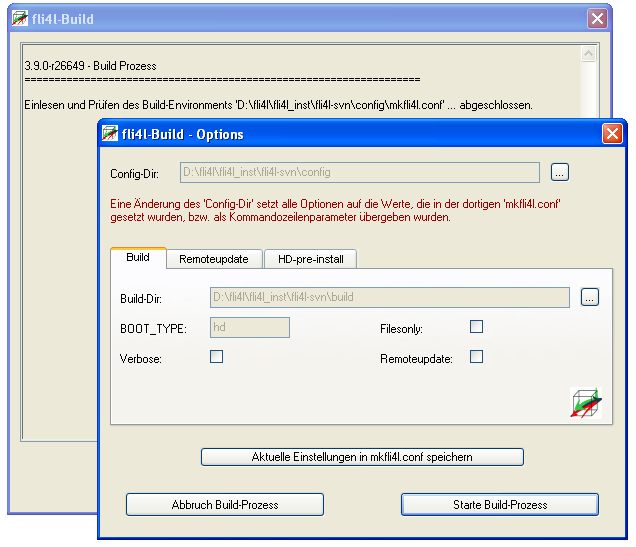
\includegraphics[width=\columnwidth]{win_build_build}
  \caption{Einstellungen}
  \label{fig:win_build_build}
  \end{figure}

  In diesem Dialog werden die Einstellungen für die Archiv/Bootmedienerstellung
  festgelegt:
  \begin{itemize}
    \item Build-Dir~-- Verzeichnis für die Archive/CD-Images/...
    \item \var{BOOT\_TYPE}~-- Anzeige des verwendeten/eingestellen \var{BOOT\_TYPE}~-- nicht änderbar
    \item Verbose~-- Aktivierung von zusätzlichen Ausgaben während der Erstellung
    \item Filesonly~-- es werden nur die Archive erstellt~-- kein bootmedium/kein Image
    \item Remoteupdate~-- Aktivierung des Remoteupdates per SCP
  \end{itemize}

  Mit der Schaltfläche \textbf{Aktuelle Einstellungen in mkfli4l.txt speichern}
  können die aktuell eingestellten Werte in der mkfli4l.txt gespeichert werden.

  \subsection{Konfigurationsdialog~-- Einstellungen für Remoteupdate}
  \begin{figure}[ht!]
  \centering
  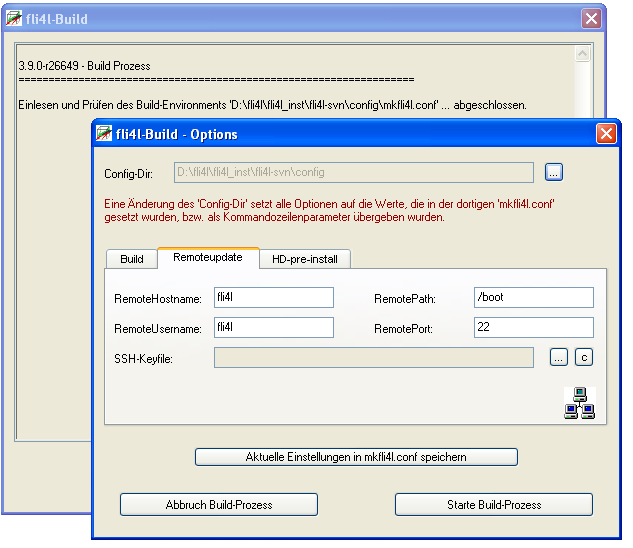
\includegraphics[width=\columnwidth]{win_build_remoteupdate}
  \caption{Einstellungen für Remoteupdate}
  \label{fig:win_build_remoteupdate}
  \end{figure}

  In diesem Dialog werden die Einstellungen für den Remoteupdate festgelegt:
  \begin{itemize}
    \item IP-Adresse oder Hostname
    \item Benutzername auf dem Remote-Host
    \item Remote-Pfad (default: /boot)
    \item Remote-Port (default: 22)
    \item zu verwendendes SSH-Keyfile (ppk-Format von Putty)
  \end{itemize}

  \subsection{Konfigurationsdialog~-- Einstellungen für HD-pre-install}
  \begin{figure}[ht!]
  \centering
  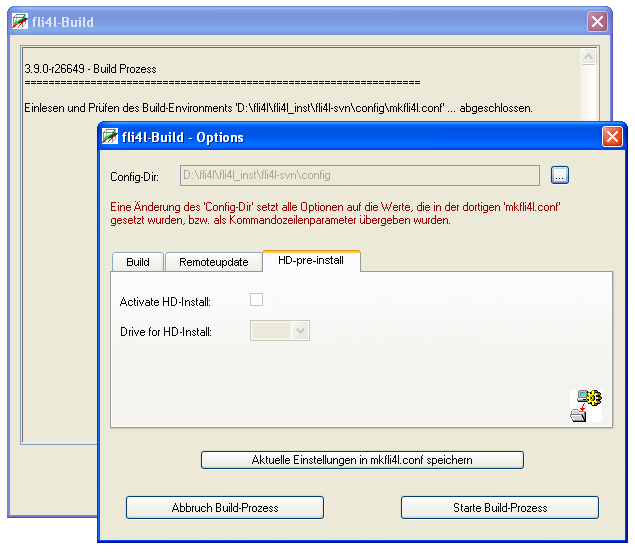
\includegraphics[width=\columnwidth]{win_build_hd_install}
  \caption{Einstellungen für HD-pre-install}
  \label{fig:win_build_hd_install}
  \end{figure}

   In diesem Dialog können die Optionen für den HD-pre-install auf einer
   entsprechend partitionierten und formatierten CompactFlash-Karte
   in einem USB-Reader eingestellt werden.

   Mögliche Optionen:
   \begin{itemize}
     \item HD-pre-install aktivieren
     \item Laufwerksbuchstabe der CF-Karte
  \end{itemize}

  Hinweis zur Partionierung und Formatierung der CF:
  Für eine HD-Installation nach TYP A (siehe dazu Paket HD) muss auf der CF eine
  primäre aktive und formatierte FAT-Partition vorhanden sein. Möchte man
  weiterhin auch eine Datenpartiton benutzen, wird zusätzlich eine Linux-Partition,
  die mit dem Dateisystem ext3 formatiert ist, sowie die Datei \texttt{hd.cfg} auf der
  FAT-Partiton benötigt (hierzu sollten unbedingt die Hinweise im Paket HD beachtet
  werden).

\marklabel{sec:mkfli4lconf}{
  \section{Steuerungsdatei mkfli4l.txt}}
  Seit fli4l-Version 2.1.9 existiert die Steuerungsdatei
  \texttt{$<$config$>$/mkfli4l.txt}. Durch sie werden z.B. vom Standard
  abweichende Verzeichnisse übergeben. Die Steuerungsdatei hat einen
  ähnlichen Aufbau wie die normalen fli4l Konfigurationsdateien.
  Alle Konfigurationsvariablen sind hier optional, d.h. sie müssen nicht
  in der Konfigurationsdatei vorkommen oder können als Kommentar gekennzeichnet
  werden.
  \begin{description}

  \config {BUILDDIR}{BUILDDIR}{BUILDDIR}

  Standardwert: `build'

  Legt fest, in welchem Verzeichnis die fli4l Dateien erzeugt werden sollen.
  Ist die Variable undefiniert, setzt mkfli4l unter Windows `build' relativ zum fli4l
  Wurzelverzeichnis ein und meint damit also das Verzeichnis
  \texttt{build} im fli4l Wurzelverzeichnis:
  \begin{verbatim}
    Pfad/fli4l-x.y.z/build
  \end{verbatim}
  \vspace{-2ex}
  Unter *nix setzt mkfli4l \texttt{$<$config$>$/build} ein und legt damit die
  generierten Dateien zusammen mit der Konfiguration ab.

  Die konfigurierten Pfade in \var{BUILDDIR} müssen der jeweiligen Logik von
  Windows oder *unix entsprechen. Werden relative Pfade gesetzt, wird der Pfad
  durch den Buildprozess passend zu Windows oder *unix konvertiert.

  \config {VERBOSE}{VERBOSE}{VERBOSE}

  Standardwert: \var{VERBOSE='no'}

  Mögliche Werte sind \var{'yes'} oder \var{'no'}. Steuert die \emph{Geschwätzigkeit}
  des Build Prozesses.

  \config {FILESONLY}{FILESONLY}{FILESONLY}

  Standardwert: \var{FILESONLY='no'}

  Mögliche Werte \var{'yes'} oder \var{'no'}. Hiermit kann das Erstellen eines
  Boot-Mediums abgeschaltet werden, es werden also nur die Dateien erzeugt~--

  \config {REMOTEUPDATE}{REMOTEUPDATE}{REMOTEUPDATE}

  Standardwert: \var{REMOTEUPDATE='no'}

  Mögliche Werte \var{'yes'} oder \var{'no'}. Aktiviert das automatische
  Übertragen der erstellten Dateien mittels SCP auf den Router. Dieses setzt
  ein installiertes Paket \jump{OPTSSHD}{SSHD} mit aktiviertem \texttt{scp}
  voraus.  Siehe dazu auch die folgenden Variablen.

  \config {REMOTEHOSTNAME}{REMOTEHOSTNAME}{REMOTEHOSTNAME}

  Standardwert: \var{REMOTEHOSTNAME=''}

  Gibt den Ziel-Hostnamen für den SCP Datentransfer an.
  Sollte kein Name angegeben sein, wird dieser der Variable
  \jump{HOSTNAME}{\var{HOSTNAME}} entnommen.

  \config {REMOTEUSERNAME}{REMOTEUSERNAME}{REMOTEUSERNAME}

  Standardwert: \var{REMOTEUSERNAME='fli4l'}

  Username für den SCP Datentransfer.

  \config {REMOTEPATHNAME}{REMOTEPATHNAME}{REMOTEPATHNAME}

  Standardwert: \var{REMOTEPATHNAME='/boot'}

  Ziel-Pfad für den SCP Datentransfer.

  \config {REMOTEPORT}{REMOTEPORT}{REMOTEPORT}

  Standardwert: \var{REMOTEPORT='22'}

  Zielport für den SCP Datentransfer.

  \config {SSHKEYFILE}{SSHKEYFILE}{SSHKEYFILE}

  Standardwert: \var{SSHKEYFILE=''}

  Hier kann man eine SSH-Keydatei für den SCP-Remoteupdate angeben.
  Es kann somit ein Update ohne Angabe eines Passwortes erfolgen.
  
  \config {REMOTEREMOUNT}{REMOTEREMOUNT}{REMOTEREMOUNT}
  
  Standardwert: \var{REMOTEREMOUNT='no'}
  
  Mögliche Werte \var{'yes'} oder \var{'no'}. Wird hier \var{'yes'}
  gesetzt, wird ein eventuell Readonly eingehängtes Bootdevice "/boot"
  für das Remoteupdate Readwrite gemountet um das Remoteupdate möglich
  zu machen. 

  \config {TFTPBOOTPATH}{TFTPBOOTPATH}{TFTPBOOTPATH}

  Pfad an dem das Netboot-Image abgelegt wird.

  \config {TFTPBOOTIMAGE}{TFTPBOOTIMAGE}{TFTPBOOTIMAGE}

  Name des Netboot-Images.

  \config {PXESUBDIR}{PXESUBDIR}{PXESUBDIR}

  Unterverzeichnis für die PXE-Dateien relativ zu TFTPBOOTPATH.


  \config {SQUEEZE\_SCRIPTS}{SQUEEZE\_SCRIPTS}{SQUEEZESCRIPTS}

   Aktiviert bzw. deaktiviert das Squeezen (Kommprimieren) von
   Skripten.
   Das Komprimieren eines Skripts mit Squeeze entfernt alle Kommentare und
   Zeileneinrückungen.
   Im Normalfall sollte hier immer der Standardwert \var{'yes'} benutzt werden.

  \config {MKFLI4L\_DEBUG\_OPTION}{MKFLI4L\_DEBUG\_OPTION}{MKFLI4LDEBUGOPTION}

   Es können zum Debuggen zusätzliche Optionen an das \jump{mkfli4l}{mkfli4l-Programm} übergeben
   werden.

  \end{description}

  \chapter{Anbindung von PCs im LAN}

  Für jeden Rechner im LAN ist einzustellen:

  \begin{enumerate}
  \item IP-Adresse (siehe \smalljump{sec:pc-lan-ip}{IP-Adresse})
  \item Name des Rechners plus Wunsch-Domain-Name
    (siehe \smalljump{sec:pc-lan-name}{Rechnername und Domain})
  \item Standard-Gateway (siehe \smalljump{sec:pc-lan-gateway}{Gateway})
  \item IP-Adresse des DNS-Servers (siehe \smalljump{sec:pc-lan-dns}{DNS-Server})
  \end{enumerate}

  \marklabel{sec:pc-lan-ip}{\section{IP-Adresse}}
  Die IP-Adresse muss im gleichen Netz wie die IP-Adresse des
  fli4l-Routers (auf Ethernet-Seite) liegen, also z.B. 192.168.6.2,
  wenn der fli4l die Adresse 192.168.6.1 hat.
  Kein Rechner darf die gleiche IP-Adresse haben, weshalb man am
  besten (nur) die letzte Zahl ändert. Auch ist darauf zu achten, dass
  man hier die gleiche IP-Adresse angibt, wie man es für diesen
  Rechner in der Datei config/base.txt angegeben hat.

  \marklabel{sec:pc-lan-name}{\section{Rechnername und Domain}}
  Der Name des Rechners ist dann z.B. ``mein-pc'', die Domain ``lan.fli4l''.

  \wichtig{Die im PC eingestellte Domain muss identisch mit der
  gewählten Domain im fli4l-Rechner sein, wenn man den fli4l-Router
  als DNS-Server verwenden will. Sonst kann es im Netz erhebliche
  Probleme geben.}

  Grund: Windows-Rechner suchen regelmäßig nach Rechnern mit dem Namen
  ihrer Arbeitsgruppte: WORKGROUP.meine-domain.fli4l. Ist dies nicht die in fli4l
  eingestellte Domain (hier: meine-domain.fli4l), wird fli4l
  versuchen, diese Anfrage durch Weiterleiten ins Internet zu
  beantworten \ldots

  Einzutragen ist die Domain in den TCP/IP Einstellungen des Rechners.

  \subsection{Windows 2000}

  Für Windows 2000 findet man das unter:

  \noindent Start \pfeil\\
  \hspace*{2ex}Einstellungen \pfeil\\
  \hspace*{4ex}Systemsteuerung \pfeil\\
  \hspace*{6ex}Netzwerk- und DFÜ-Verbindungen \pfeil\\
  \hspace*{8ex}LAN-Verbindung \pfeil\\
  \hspace*{10ex}Eigenschaften \pfeil\\
  \hspace*{12ex}Internetprotokoll (TCP/IP) \pfeil\\
  \hspace*{14ex}Eigenschaften \pfeil\\
  \hspace*{16ex}Erweitert\ldots \pfeil\\
  \hspace*{18ex}DNS \pfeil\\
  \hspace*{20ex}DNS-Suffix hinzufügen \pfeil\\

  ``lan.fli4l'' (bzw. die eingestellte domain) eingeben (ohne ``''!)
  \pfeil OK drücken.

\subsection{NT 4.0}

  Start \pfeil\\
  \hspace*{2ex}Einstellungen \pfeil\\
  \hspace*{4ex}Systemsteuerung  \pfeil\\
  \hspace*{6ex}Netzwerk \pfeil\\
  \hspace*{8ex}Protokolle \pfeil\\
  \hspace*{10ex}TCP/IP \pfeil\\
  \hspace*{12ex}Eigenschaften \pfeil\\
  \hspace*{14ex}DNS \pfeil\\
  \hspace{16ex}\begin{itemize}
  \item Hostname eintragen (eigener Rechnername)
  \item Domäne eintragen (wie in config/base.txt)
  \item IP-Adresse vom fli4l-Router hinzufügen
  \item DNS-Suffix hinzufügen (Domäne hinzufügen~-- siehe
    2 Zeilen höher)
  \end{itemize}

\subsection{Win95/98}

  Start \pfeil\\
  \hspace*{2ex}Einstellungen \pfeil\\
  \hspace*{4ex}Systemsteuerung \pfeil\\
  \hspace*{6ex}Netzwerk \pfeil\\
  \hspace*{8ex}Konfiguration \pfeil\\
  \hspace*{10ex}TCP/IP (jenes, das an die Netzwerkkarte zum Router\\
  \hspace*{10ex}angebunden ist) \pfeil\\
  \hspace*{12ex}Eigenschaften \pfeil\\
  \hspace*{14ex}DNS-Konfiguration:

  DNS aktivieren und bei ``Domäne:'' dann ``lan.fli4l'' eingeben (ohne ``''!).

\subsection{Windows XP}

  Für Windows XP findet man das unter:

  \noindent Start \pfeil\\
  \hspace*{2ex}Einstellungen \pfeil\\
  \hspace*{4ex}Systemsteuerung \pfeil\\
  \hspace*{6ex}Netzwerkverbindungen \pfeil\\
  \hspace*{8ex}LAN-Verbindung \pfeil\\
  \hspace*{10ex}Eigenschaften \pfeil\\
  \hspace*{12ex}Internetprotokoll (TCP/IP) \pfeil\\
  \hspace*{14ex}Eigenschaften \pfeil\\
  \hspace*{16ex}Erweitert\ldots \pfeil\\
  \hspace*{18ex}DNS \pfeil\\
  \hspace*{20ex}DNS-Suffix für diese Verbindung \pfeil\\

  ``lan.fli4l'' (bzw. die eingestellte domain) eingeben (ohne ``''!)
  \pfeil OK drücken.

\subsection{Windows 7}

  Für Windows 7 findet man das unter:

  \noindent Windows Button (ex. Start) \pfeil\\
  \hspace*{2ex}Systemsteuerung \pfeil\\
  \hspace*{4ex}Netzwerk und Internet \pfeil\\
  \hspace*{6ex}Netzwerk- und Freigabecenter \pfeil\\
  \hspace*{8ex}LAN-Verbindung \pfeil\\
  \hspace*{10ex}Eigenschaften \pfeil\\
  \hspace*{12ex}Internetprotokoll Version 4 (TCP/IPv4) \pfeil\\
  \hspace*{14ex}Eigenschaften \pfeil\\
  \hspace*{16ex}Erweitert\ldots \pfeil\\
  \hspace*{18ex}DNS \pfeil\\
  \hspace*{20ex}DNS-Suffix für diese Verbindung \pfeil\\

  ``lan.fli4l'' (bzw. die eingestellte domain) eingeben (ohne ``''!)
  \pfeil OK drücken.

\subsection{Windows 8}

  Für Windows 8 findet man das unter:

  \noindent Gleichzeitig Windows- und X-Taste drücken \pfeil\\
  \hspace*{2ex}Systemsteuerung \pfeil\\
  \hspace*{4ex}Netzwerk und Internet \pfeil\\
  \hspace*{6ex}Netzwerk- und Freigabecenter \pfeil\\
  \hspace*{8ex}Ihr Netzwerk wählen (Ehternet oder WLAN) \pfeil\\
  \hspace*{10ex}Eigenschaften \pfeil\\
  \hspace*{12ex}Internetprotokoll Version 4 (TCP/IPv4) \pfeil\\
  \hspace*{14ex}Eigenschaften \pfeil\\
  \hspace*{16ex}Erweitert\ldots \pfeil\\
  \hspace*{18ex}DNS \pfeil\\
  \hspace*{20ex}DNS-Suffix für diese Verbindung \pfeil\\

  ``lan.fli4l'' (bzw. die eingestellte domain) eingeben (ohne ``''!)
  \pfeil OK drücken.

  \marklabel{sec:pc-lan-gateway}{\section{Gateway}}
  Die Angabe des Standard-Gateways ist unbedingt erforderlich, denn
  ohne die Angabe der richtigen IP-Adresse an dieser Stelle
  funktioniert nichts.  Es muß hier die IP-Adresse des fli4l-Routers
  (auf Ethernet-Seite) angegeben werden, also z.B. 192.168.6.4
  entsprechend der IP-Adresse, die hier in der Datei config/base.txt
  für den fli4l-Router angegeben wurde.

  Es ist falsch, den fli4l-Router als Proxy in der Windows- oder
  Browser- Konfiguration einzutragen~-- außer man setzt ein Proxy auf
  dem fli4l-Router ein. Im Normalfall ist fli4l kein Proxy, daher
  bitte \emph{nicht} fli4l als Proxy angeben!

\marklabel{sec:pc-lan-dns}{\section{DNS-Server}}

  Als IP-Adresse des DNS-Servers gibt man nicht die Adresse des
  Provider-DNS-Servers an, sondern die des fli4l-Routers (Ethernet),
  da dieser nun selbst Anfragen beantworten kann bzw. diese bei
  Unkenntnis ins Internet weiterleitet.

  Mit der Konstruktion von fli4l als DNS-Server werden viele von den
  Windows-PCs ausgeführten Anfragen nicht ins Internet weitergeroutet,
  sondern werden direkt vom fli4l-Router beantwortet.

\marklabel{sec:pc-lan-misc}{\section{Verschiedenes}}

  Die Punkte 1 bis 4 brauchen bei konfiguriertem DHCP-Server nicht
  eingetragen zu werden, da dann der fli4l-Router die notwendigen Daten
  automatisch übermittelt.

  \textbf{Internetoptionen:} Bei Verbindungen muß ``keine Verbindung wählen'' ausgewählt sein.
  Bei Einstellungen für lokales Netzwerk(LAN): es darf hier NICHTS
  angegeben werden (es sei dann es wird \var{OPT\_\-P}roxy verwendet).
  Beides sind Standardeinstellungen, die im Normalfall nicht geändert
  werden müssen.

\marklabel{IMONDSCHNITTSTELLE}{
    \chapter{Client-/Server-Schnittstelle imon}
  }

  \marklabel{sec:imond}{
    \section{imon-Server imond}}

  imond ist ein netzwerkfähiges Server-Programm, welches bestimmte
  Anfragen beantwortet oder auch Kommandos zur Steuerung des Routers
  entgegennehmen kann.

  Ausserdem steuert imond das Least-Cost-Routing. Dazu verwendet er
  eine Konfigurationsdatei /etc/imond.conf, welche beim Booten
  automatisch aus den \var{ISDN\_\-CIRC\_\-x\_\-XXX}-Variablen der Datei
  config/isdn.txt und anderen über ein Shell-Script erzeugt wird.

  imond läuft permanent als Daemon und horcht gleichzeitig auf
  TCP/IP-Port 5000 und Device /dev/isdninfo.

  Folgende Kommandos sind über den TCP/IP-Port 5000 möglich:
  \begin{table}
    \textbf{Admin-Befehle}

    \vspace{1ex}
    \begin{tabular}{lp{9cm}}

      addlink ci-index              & Channel zum Circuit hinzufügen
                                      (Channel-Bundling) \\
      adjust-time seconds           & Ändert die Uhrzeit des Routers um die
                                      angegebenen Sekunden \\
      delete filename pw            & Löscht die Datei auf dem Router \\
      hup-timeout \#ci-index [value]& Anzeigen bzw. Setzen des HUP-Timeout für
                                      ISDN-Circuits \\
      removelink ci-index           & Zusätzlichen Channel wieder entfernen \\
      reset-telmond-log-file        & Löschen der telmond-Protokolldatei \\
      reset-imond-log-file          & Löschen der imond-Protokolldatei \\
      receive filename \#bytes pw   & Eine Datei auf den Router übertragen.
                                      Dazu quittiert imond den Befehl mit
                                      einem ACK (0x06). Danach wird die Datei
                                      in 1024er-Blöcken übertragen, die imond
                                      auch jeweils mit einem ACK bestätigt.
                                      Als letztes übermittelt imond noch ein
                                      OK. \\
      send filename pw              & Wenn das Passwort stimmt und die Datei
                                      existiert, liefert imond ein OK \#bytes.
                                      Anschliessend überträgt imond die Datei
                                      in 1024er Blöcken, die jeweils mit
                                      einem ACK (0x06) bestätigt werden
                                      müssen. Als letztes liefert imond noch
                                      ein OK. \\
      support pw                    & Liefert den Status/Konfiguration vom
                                      Router \\
      sync                          & Synchronisiert den Cache von gemounteten
                                      Laufwerken \\
    \end{tabular}
  \end{table}


  \begin{table}
    \textbf{Admin- oder User-Befehle}

    \vspace{1ex}
    \begin{tabular}{lp{9cm}}

      dial                      &    Wählt den Provider an
                                     (Default-Route-Circuit) \\
      dialmode [auto|manual|off]&    Liefert bzw. setzt den Dialmode \\
      disable                   &    Hängt ein und setzt dialmode auf ``off''
                                      \\
      enable                    &    Setzt dialmode auf ``auto'' \\
      halt                      &    Fährt den Router sauber herunter \\
      hangup [\#channel-id]     &    Hängt ein \\
      poweroff                  &    Fährt den Router herunter und schaltet ab \\
      reboot                    &    Reboot vom i4l-Router! \\
      route [ci-index]          &    Setzen Default-Route auf Circuit X
                                     (0=automatisch) \\
    \end{tabular}
  \end{table}


  \begin{table}
    \textbf{User-Befehle}

    \vspace{1ex}
    \begin{tabular}{lp{9cm}}
      channels                  & Ausgabe Anzahl der verfügbaren ISDN-Kanäle\\
      charge \#channel-id       & Ausgabe der Online-Kosten für einen
                                  Channel\\
      chargetime \#channel-id   & Online-Zeit unter Berücksichtigung des
                                  Taktes\\
      circuit [ci-index]        & Ausgabe eines Circuit-Namens\\
      circuits                  & Ausgabe Anzahl der Default-Route-Circuits\\
      cpu                       & Liefert die Auslastung der CPU in Prozent\\
      date                      & Ausgabe Datum/Uhrzeit\\
      device ci-index           & Liefert das Device des Circuits\\
      driverid \#channel-id     & Ausgabe Driver-Id für Channel X\\
      help                      & Ausgabe Hilfe\\
      inout \#channel-id        & Ausgabe der Richtung (incoming/outgoing)\\
      imond-log-file            & Ausgabe imond-Protokolldatei\\
      ip \#channel-id           & Ausgabe der IP\\
      is-allowed command        & Ausgabe, ob Befehl konfiguriert/gültig
                                  ist\newline
                                  Mögliche Befehle:
                                    dial|dialmode|route|reboot|
                                    imond-log|telmond-log|mgetty-log \\
      is-enabled                & Ausgabe, ob dialmode auf off (0) oder auto
                                  (1)\\
      links ci-index            & Ausgabe Anzahl momentaner Channel 0, 1 oder
                                  2, 0 heisst: Kein Channel-Bundling möglich\\
      log-dir imond|telmond|mgetty& Liefert das Logverzeichnis\\
      mgetty-log-file           & Ausgabe mgetty-Protokolldatei\\
      online-time \#channel-id  & Ausgabe Online-Zeit der akt. Verbindung in
                                  hh:mm:ss\\
      pass [password]           & Abfrage, ob Password nötig bzw. Password-
                                  Eingabe\newline
                                  1 Userpassword gesetzt\newline
                                  2 Adminpassword gesetzt\newline
                                  4 imond befindet sich im Admin-Modus\\
      phone \#channel-id        & Ausgabe Telefonnummer/Name des ``Gegners''\\
      pppoe                     & Liefert die Anzahl der pppoe-Devices (also 0
                                  oder 1)\\
      quantity \#channel-id     & Liefert die übertragenen Datenmengen (in
                                  Byte)\\
      quit                      & Beenden der Verbindung zu imond\\
      rate \#channel-id         & Ausgabe Übertragungsraten (incoming/outgoing
                                  in B/sec)\\
      status \#channel-id       & Ausgabe Status für Channel X\\
      telmond-log-file          & Ausgabe telmond-Protokolldatei\\
      time \#channel-id         & Ausgabe Summe Online-Zeiten, Format
                                  hh:mm:ss\\
      timetable [ci-index]      & Ausgabe der Zeittabelle für LC-Routing\\
      uptime                    & Ausgabe der Uptime des Routers in Sekunden\\
      usage \#channel-id        & Ausgabe Art der Verbindung, mögliche
                                  Antworten: Fax, Voice, Net, Modem, Raw\\
      version                   & Ausgabe der Protokoll- und
                                  Programm-Version\\
    \end{tabular}
  \end{table}


  Der TCP/IP-Port 5000 ist nur vom maskierten LAN aus erreichbar.
  Standardmäßig wird ein Zugriff von aussen über die
  Firewall-Konfiguration abgeblockt.

  Imond unterstützt zwei Benutzerebenen: den User- und den
  Admin-Modus.  Für beide Ebenen kann ein Passwort gesetzt werden
  mittels \var{IMOND\_\-PASS} bzw.  \var{IMOND\_ADMIN\_\-PASS}. Dadurch
  werden die imon-Clients von imond gezwungen, eine Password-Abfrage
  durchzuführen und anschließend das Password an imond zu übertragen.
  Solange dieses Password nicht übermittelt wurde, nimmt imond nur die
  beiden Kommandos ``pass'' und ``quit'' entgegen. Alle anderen werden
  mit einem Fehler zurückgewiesen.

  Möchte man das weiter einschränken, z.B. den Zugriff nur von nur
  einem PC erlauben, muss die Firewall-Konfiguration angepasst werden.

  Die Befehle

\begin{example}
\begin{verbatim}
         enable/disable/dialmode   dial/hangup   route   reboot/halt
\end{verbatim}
\end{example}

  können durch die Konfigurationsvariablen \var{IMOND\_\-XXX} global ein- oder
  abgeschaltet werden (s. Kapitel ``Konfiguration'').

  Mit einem Unix/Linux-Rechner (oder einem Windows-Rechner in der DOS-Box)
  kann man das Ganze leicht ausprobieren:

  Nach Eingabe von

\begin{example}
\begin{verbatim}
        telnet fli4l 5000        \# oder entsprechender Name des fli4l-Routers
\end{verbatim}
\end{example}

  kann man direkt die oben aufgeführten Kommandos eingeben und sich
  die Ausgabe anschauen.

  Zum Beispiel bekommt man mit ``help'' die Hilfe angezeigt, mit
  ``quit'' wird die Verbindung zum imond abgebaut.

\marklabel{sec:leastcostrouting}{
  \subsection{Least-Cost-Routing~-- Funktionsweise}
  }

  imond konstruiert aus der Konfigurationsdatei /etc/imond.conf
  (welche wiederum beim Booten aus den Konfigurationsvariablen
  \var{ISDN\_\-CIRC\_\-x\_\-TIMES} usw.  erstellt wird), eine zeitabhängige
  Tabelle (Time-Table). Diese umfasst eine komplette Kalenderwoche im
  1-Stunden-Raster (168 Stunden = 168 Bytes). Die Tabelle setzt sich
  jedoch lediglich aus Circuits zusammen, für die eine Default-Route
  definert ist.

  Mit dem imond-Kommando ``timetable'' kann man sich diese Tabelle
  anschauen.

  Hier ein Beispiel:

  Nehmen wir an, dass 3 Circuits definiert wurden, nämlich:

\begin{example}
\begin{verbatim}
        CIRCUIT_1_NAME='Addcom'
        CIRCUIT_2_NAME='AOL'
        CIRCUIT_3_NAME='Firma'
\end{verbatim}
\end{example}

  wobei lediglich die ersten beiden Circuits mit Default-Routen belegt
  sind, also die enstprechenden Variablen ISDN\_CIRC\_x\_ROUTE den
  Wert `0.0.0.0' haben.

  Wenn die dazugehörigen Variablen \var{ISDN\_\-CIRC\_\-x\_\-TIMES} folgendermaßen
  aussehen:

\begin{example}
\begin{verbatim}
        ISDN_CIRC_1_TIMES='Mo-Fr:09-18:0.0388:N Mo-Fr:18-09:0.0248:Y
                      Sa-Su:00-24:0.0248:Y'

        ISDN_CIRC_2_TIMES='Mo-Fr:09-18:0.019:Y Mo-Fr:18-09:0.049:N
                      Sa-Su:09-18:0.019:N Sa-Su:18-09:0.049:N'

        ISDN_CIRC_3_TIMES='Mo-Fr:09-18:0.08:N Mo-Fr:18-09:0.03:N
                      Sa-Su:00-24:0.03:N'
\end{verbatim}
\end{example}

  dann wird daraus folgende Datei /etc/imond.conf:

\begin{example}
\begin{verbatim}
        #day  hour  device  defroute  phone        name        charge  ch-int
        Mo-Fr 09-18 ippp0   no        010280192306 Addcom      0.0388   60
        Mo-Fr 18-09 ippp0   yes       010280192306 Addcom      0.0248   60
        Sa-Su 00-24 ippp0   yes       010280192306 Addcom      0.0248   60
        Mo-Fr 09-18 ippp1   yes       019160       AOL  0.019   180
        Mo-Fr 18-09 ippp1   no        019160       AOL  0.049   180
        Sa-Su 09-18 ippp1   no        019160       AOL  0.019   180
        Sa-Su 18-09 ippp1   no        019160       AOL  0.049   180
        Mo-Fr 09-18 isdn2   no        0221xxxxxxx  Firma       0.08     90
        Mo-Fr 18-09 isdn2   no        0221xxxxxxx  Firma       0.03     90
        Sa-Su 00-24 isdn2   no        0221xxxxxxx  Firma       0.03     90
\end{verbatim}
\end{example}

  imond erstellt dann im Speicher folgende Time-Table~-- hier die Ausgabe
  über das imond-Kommando ``timetable'':

\begin{example}
\begin{verbatim}
         0  1  2  3  4  5  6  7  8  9 10 11 12 13 14 15 16 17 18 19 20 21 22 23
     --------------------------------------------------------------------------
     Su  3  3  3  3  3  3  3  3  3  3  3  3  3  3  3  3  3  3  3  3  3  3  3  3
     Mo  2  2  2  2  2  2  2  2  2  4  4  4  4  4  4  4  4  4  2  2  2  2  2  2
     Tu  2  2  2  2  2  2  2  2  2  4  4  4  4  4  4  4  4  4  2  2  2  2  2  2
     We  2  2  2  2  2  2  2  2  2  4  4  4  4  4  4  4  4  4  2  2  2  2  2  2
     Th  2  2  2  2  2  2  2  2  2  4  4  4  4  4  4  4  4  4  2  2  2  2  2  2
     Fr  2  2  2  2  2  2  2  2  2  4  4  4  4  4  4  4  4  4  2  2  2  2  2  2
     Sa  3  3  3  3  3  3  3  3  3  3  3  3  3  3  3  3  3  3  3  3  3  3  3  3

     No.  Name                   DefRoute  Device  Ch/Min   ChInt
      1   Addcom                   no      ippp0   0.0388     60
      2   Addcom                   yes     ippp0   0.0248     60
      3   Addcom                   yes     ippp0   0.0248     60
      4   AOL               yes     ippp1   0.0190    180
      5   AOL               no      ippp1   0.0490    180
      6   AOL               no      ippp1   0.0190    180
      7   AOL               no      ippp1   0.0490    180
      8   Firma                    no      isdn2   0.0800     90
      9   Firma                    no      isdn2   0.0300     90
     10   Firma                    no      isdn2   0.0300     90
\end{verbatim}
\end{example}

  Für den Circuit 1 (Addcom) sind also drei Zeitbereiche (1-3)
  eingetragen, für Circuit 2 (AOL) vier Zeitbereiche (4-7) und
  für den letzen drei Zeitbereiche (8-10).

  In der Time-Table werden jeweils die Indices ausgegeben, welche für
  die jeweilige Stunde gültig sind. Hier tauchen lediglich die Indices
  2-4 auf, da alle anderen keine LC-Default-Routen sind.

  Sieht man in der Tabelle irgendwo Nullen, gibt es Lücken in den
  \var{ISDN\_\-CIRC\_\-X\_\-TIMES}-Werten. Dann existiert zu diesen Zeiten keine
  Default-Route, Internet-Zugang abgeknipst!

  Beim Programmstart ermittelt imond zunächst den Wochentag und die
  aktuelle Stunde. Anschließend wird dann über die Time-Table der
  Index ermittelt und damit dann auch der entsprechende Circuit. Auf
  diesen wird dann die Default-Route gesetzt.

  Bei Zustandsänderungen der Channels, z.B. Wechsel von online
  nach offline~-- jedoch spätestens nach 1 Minute~-- geht das Spiel von
  neuem los: Zeit ermitteln, Lookup in Tabelle, Default-Route-Circuit
  ermitteln.

  Ändert sich der aktuell verwendete Circuit, z.B. montags um 18:00
  Uhr, wird die alte Default-Route gelöscht, eine vielleicht
  bestehende Verbindung beendet (sorry\ldots) und anschließend die
  Default-Route auf den neuen Circuit gesetzt. Dies kann von imond bis
  zu 60 Sekunden später bemerkt werden, also wird spätestens um
  18:00:59 umgeschaltet.

  Bei Circuits, die keine Default-Route belegen, ändert sich überhaupt
  nichts. Hier wird der Inhalt von \var{ISDN\_\-CIRC\_\-x\_\-TIMES} lediglich zur
  Berechnung der Telefonkosten verwendet. Diese können dann relevant
  sein, wenn man über den Client imonc das LC-Routing temporär
  ausschaltet und einen Circuit manuell wählt.

  Man kann sich jedoch auch die Tabellen für andere
  Zeitbereich-Indices (im Beispiel von 1 bis 10) anschauen, auch die
  der ``Non-LC-Default-Route-Circuits''.

  Kommando:

\begin{example}
\begin{verbatim}
                    timetable index
\end{verbatim}
\end{example}

  Beispiel:

\begin{example}
\begin{verbatim}
                    telnet fli4l 5000
                    timetable 5
                    quit
\end{verbatim}
\end{example}

  Die Ausgabe sieht dann so aus:

\begin{example}
\begin{verbatim}
         0  1  2  3  4  5  6  7  8  9 10 11 12 13 14 15 16 17 18 19 20 21 22 23
     --------------------------------------------------------------------------
     Su  0  0  0  0  0  0  0  0  0  0  0  0  0  0  0  0  0  0  0  0  0  0  0  0
     Mo  5  5  5  5  5  5  5  5  5  0  0  0  0  0  0  0  0  0  5  5  5  5  5  5
     Tu  5  5  5  5  5  5  5  5  5  0  0  0  0  0  0  0  0  0  5  5  5  5  5  5
     We  5  5  5  5  5  5  5  5  5  0  0  0  0  0  0  0  0  0  5  5  5  5  5  5
     Th  5  5  5  5  5  5  5  5  5  0  0  0  0  0  0  0  0  0  5  5  5  5  5  5
     Fr  5  5  5  5  5  5  5  5  5  0  0  0  0  0  0  0  0  0  5  5  5  5  5  5
     Sa  0  0  0  0  0  0  0  0  0  0  0  0  0  0  0  0  0  0  0  0  0  0  0  0

     No.  Name                   DefRoute  Device  Ch/Min   ChInt
      5   AOL               no      ippp1   0.0490    180
\end{verbatim}
\end{example}

  Alles klar?

  Mit dem imond-Kommando ``route'' kann das LC-Routing ein- und
  ausgeschaltet werden. Bei Angabe eines positiven Circuit-Indices
  (1\ldots N) wird die Default-Route auf den angegebenen Circuit
  gelegt. Ist der Index 0, wird das LC-Routing wieder aktiviert und
  der Circuit automatisch ausgewählt.


  \subsection{Zur Berechnung der Onlinekosten}

  Das ganze Modell zur Berechnung der Onlinekosten funktioniert nur
  korrekt, wenn der Zeittakt für einen Circuit (Variable
  \var{ISDN\_\-CIRC\_\-x\_\-CHARGEINT}) über die ganze Woche konstant ist. Dies
  ist im Normalfall bei Internet-Providern die Regel. Wählt man sich
  jedoch über die Telekom (ich meine nicht T-Online!) z.B. in sein
  Firmennetz ein, gilt das als ganz normales Telefongespräch. Und da
  wechselt ab 18:00 der Takt von 90 Sekunden auf 4 Minuten (Stand Juni
  00). Deshalb ist die Definition von

\begin{example}
\begin{verbatim}
        ISDN_CIRC_3_CHARGEINT='90'
        ISDN_CIRC_3_TIMES='Mo-Fr:09-18:0.08:N Mo-Fr:18-09:0.03:N Sa-Su:00-24:0.03:N'
\end{verbatim}
\end{example}

  eigentlich nicht ganz korrekt. Es sind zwar abends umgerechnet auf
  die Minute 3 Pfennig (4 Minuten kosten 12 Telekom-Pfennige), jedoch
  ist der Takt falsch. Deshalb können bei der Kostenanzeige
  Differenzen zu den tatsächlichen Zahlen auftreten.

  Hier ist ein Tipp, wie verschieden lange Taktzeiten dennoch richtig
  berücksichtigt werden können (auch wichtig für
  \var{ISDN\_\-CIRC\_\-x\_\-CHARGEINT}): Man definiert einfach 2 Circuits,
  einen für tagsüber mit \var{ISDN\_\-CIRC\_\-1\_\-CHARGEINT}=`90' und den
  anderen mit \var{ISDN\_\-CIRC\_\-2\_\-CHARGEINT}=`240'.
  Natürlich muss man dann auch noch \var{ISDN\_\-CIRC\_\-x\_\-TIMES}
  entsprechend wählen, damit tagsüber Circuit 1 und abends Circuit 2
  verwendet wird.

  Wie gesagt: Bei Nutzung von Verbindungen zu Internet-Providern gibt
  es das Problem nicht, weil dort der Zeittakt immer konstant ist und
  lediglich die Kosten pro Minute wechseln (oder gibt es sowas doch???
  Ich traue T-* alles zu :-).

  % Synchronized to r30003
  \marklabel{sec:winimonc}{
    \section{Windows-Client imonc.exe}}

  \subsection{Introduction}

  imond on the router and on the client imonc as a team have
  two use modes: the user and the admin mode. In admin mode, all
  controls are enabled. In user mode the variables
  \jump{IMONDENABLE}{\var{IMOND\_ENABLE}}, \jump{IMONDDIAL}{\var{IMOND\_DIAL}}, 
  \jump{IMONDROUTE}{\var{IMOND\_ROUTE}} and \jump{IMONDREBOOT}{\var{IMOND\_REBOOT}}
  control if the respective functions are available. If all of these
  variables are set to `no ', this means that all buttons in the overview page
  are disabled except for the exit and the admin mode button. The
  decision whether the user or admin mode is used, is based on the
  transmitted password. By clicking the button admin mode, located in the
  status bar, you may switch to the admin mode at any time by entering the
  admin password. To switch back imonc must be restarted.

  Once imonc is started an additional tray icon is displayed, which
  shows the connection status of existing channels.

  The colors mean:
  \begin{description}
    \item[Red]: Offline
    \item[Yellow]: A connection is in the process of being established
    \item[Light Green]: Online and traffic on the channel
    \item[Dark Green]: Online and (nearly) no traffic on the channel
  \end{description}

  \noindent imonc shows a behavior a little different from the Windows standard
  when clicking on the minimize button in the title bar. This minimizes imonc
  to the system tray only a tray icon near the clock remains. Double clicking
  on the tray icon with the left mouse button brings imonc's window back to
  the foreground. With the right mouse button you may use the context menu,
  of the tray icon to execute the main imonc commands die angezeigten
         without displaying its
  main window.

  Imonc stores many properties (including all columns widths of the string grids)
  in the registry, so its appearance may be widely adapted to your needs. Imonc
  uses the registry key HKCU{\textbackslash}Software{\textbackslash}fli4l
  to store this informations

  If even after careful reading of the documentation problems on imonc or the
  router itself still remain you can post to the newsgroup. It makes sense
  to note the support information you get when choosing SystemInfo and then Info
  on the About page of the imonc client. The router password will be queried
  then (not the imond password) and after that imonc will create a file fli4lsup.txt
  that contains all the important information regarding the router, including
  imonc. This file can be posted on the newsgroup when explicitely demanded
  and will give much better chance for quick help.

  Further details concerning the development of the Windows imonc client can be found
  on the homepage of Windows Imonc \altlink{http://www.imonc.de/}. Here you can
  see what new features and bug fixes will be included in the next version.
  In addition, you will find the latest imonc version, if it is not included
  in the FLI4L distribution already.

  \subsection{Start Parameters}

  Imonc requires the name or IP address of the router fli4l. As the default
  the program attempts to establish a connection with the computer ``fli4l''.
  If this entry is correctly entered in the DNS, this should work out of the box.
  Otherwise you can pass following parameters in the link:

  \begin{itemize}
    \item /Server:The router's IP or hostname (short form: /S:IP or hostname)
    \item /Password:password (short form: /P:password)
    \item /log Option for logging communication betweeen imonc und imond. When
      entered a file imonc.log  will be written each time when imonc exits. It
      contains the complete communication and thus can grow quite large. Please
      use this parameter only in case of problems.
    \item /iport:Portnumber Portnumber imond listens to. Default: 5000
    \item /tport:Portnummer Portnumber telmond listens to. Default: 5001
    \item /rc:''Command'' The command provided here will be transmitted to the
      router without further checking and imonc will exit afterwards. 
      If more than one command should be transmitted at once, they must be devided
      by semicolons. You will have to provide an imond password in addition for
      this to work because no password query will be queried. Possible command
      are documented with imond, see chapter 8.1. In addition to the commands
      there another one exists: timesync. If used imonc will synchronize the
      clock of the client with the router's clock. The command dialtimesync is
      not supported anymore, it is substituted by "dial; timesync".
    \item /d:''fli4l-Directory'' Pass the fli4l-directory as a start parameter.
      May be of interest when using more than one fli4l version.
    \item /wait If the hostname can't be reolved imonc will not exit anymore~--
      start another try by doubleclicking the tray icon.
    \item /nostartcheck Disables checking of imonc already running. Only makes
      sense to monitor several different fli4l routers in a net. When using more
      instances the builtin syslog- and \mbox{E-Mail}-capabilites will be disabled.
  \end{itemize}

  Usage (to be entered in the link):

\begin{example}
\begin{verbatim}
X:\...imonc.exe [/Server:Host] [/Password:Password] [/iport:Portnumber]
            [/log] [/tport:Portnumber] [/rc:"Command"]
\end{verbatim}
\end{example}

  Example with IP address:

\begin{example}
\begin{verbatim}
        C:\wintools\imonc /Server:192.168.6.4
\end{verbatim}
\end{example}

  or with name and password:

\begin{example}
\begin{verbatim}
        C:\wintools\imonc /S:fli4l /P:secret
\end{verbatim}
\end{example}

  or with name and password and router command:

\begin{example}
\begin{verbatim}
        C:\wintools\imonc /S:fli4l /P:secret /rc:"dialmode manual"
\end{verbatim}
\end{example}

  \subsection{Overview}

  The Windows client queries some imond information on the existing
  connections and displays it in its window. In addition to general
  status information such as uptime of the router or the time (both locally
  and on the router), for each existing connection the following informations
  are shown:

  \begin{tabular}{lp{9cm}}
    Status             &Connection establishment/Online/Offline\\
    Name               &Telephone number of the caller or circuit name\\
    Direction          &Indicates if a connection is incoming or outgoing\\
    IP                 &IP, that was assigned to the router\\
    IBytes             &Bytes received\\
    OBytes             &Bytes sent\\
    Online time        &Actual online time\\
    Time               &Sum of all online times\\
    KTime              &Sum of all online times in consideration of charge intervals\\
    Cost               &Computed costs\\
  \end{tabular}

  \medskip

  The data is updated every 2 seconds by default. In the context menu of
  this overview it is possible to copy the assigned IP to the clipboard
  as well as hanging up the channel (for each available channel which is
  online at the moment). This is of interest in case that several different
  connections exist, e.g. one to surf the Internet and another to a private
  net and only one of them should be terminated.

  If the telmond process is active on the router, imonc can show information
  about incoming phone calls (ie calling and called MSN) in addition. The last
  incoming phone call is displayed above the buttons. a log of phone calls received
  can be obtained by viewing the calls page.

  By the six buttons in imonc the following commands can be selected:

  \begin{tabular}{clp{9cm}}
    Button & Caption & Function \\
    1& Connect/Disconnect &   Dial/Hang up\\
    2& Add link/Rem link  &   Bundle channels: yes/no~-- only available in admin mode\\
    3& Reboot             &   Reboot fli4l!\\
    4& PowerOff           & Shut down fli4l and power off afterwards\\
    5& Halt               & Shut down fli4l to power off safe afterwards\\
    6& Exit               & Exit client\\
  \end{tabular}

  \medskip

  \noindent The first five commands can be switched on and off individually in the
  router's configuration file config/base.txt for the user mode. In admin mode all
  are enabled. The dialmode controls the dialing behavior of the router:

  \begin{tabular}{lp{9cm}}
    Auto  & The router will establish connections automatically when getting 
    queries from the local net for the circuit concerned.\\
    Manual & The user himself has to establish connections.\\
    Off   & No connections can be established. The dial button is deactivated.\\
  \end{tabular}

  \medskip

  \noindent Note that fli4l by default will dial out independently. So you never
  actually will have to press the connect button\ldots

  It is also possible to manually switch the default route circuit, setting
  the automatic LCR on and off. In the Windows version of imonc the selection
  list `` default route'' is provided for this. In addition you can configure the
  hangup TimeOut time directly in imonc. use the Config button next to the default
  route for this. All configured circuits of the router are displayed here. The
  value in the column Hup-timeout can be edited directly in the string grid
  for ISDN circuits (not yet working for DSL).

  An overview over LCR can be found on the page admin/Timetable.
  There you'll see what circuit imond selects automatically at which time.

  \subsection{Config-Dialog}

  The configuration is reached using the Config button in the status bar. The window
  is divided into the following areas:

  \begin{itemize}
  \item The Area General:
    \begin{itemize}
    \item Actualization Interval: Set here how often the overview should get actualized.
    \item Synchronize Time on Startup: When starting the client's system time and date 
      will get synchronized with the router's system time. You can execute this manually
      by using the button Synchronize on the Overview-page.
    \item Start Minimized: Program will start minimized to the system tray.
    \item Start with Windows: Specify here if the client should start automatically 
      with system start. Provide necessary start-parameters in the field Parameter.
    \item Fetch News from fli4l.de: Should news from fli4l's homepage be fetched and
      displayed by imonc? Then headlines are shown in the status bar. A new page News
      is displayed to show the complete messages.
    \item Logfile for Connections: The file name here is used to save connection lists
      locally on the imonc's system.
    \item TimeOut for router to answer: How long should we wait for an answer from the
      router before assuming that the connection has failed.
    \item Language: Pick the language for imoncs to use.
    \item Confirm Router Commands: If activated all commands influencing the router
      generally have to be confirmed, i.e. Reboot, Hangup \ldots
    \item Hang up even when traffic: No information should be displayed when the
      connection is closed and there is still traffic on the line.
    \item Automatic Connection to the router: Should we try to reconnect to the router
      in case of lost connections (i.e. when rebooting the router).
    \item Minimize Window To System Tray: Should imonc minimize to system tray instead
      of terminating itself when clicking the Exit button.
    \end{itemize}

  \item Proxy Settings:
    Define a proxy for imonc's http-queries here. It will be used for fetching news.
    \begin{itemize}
    \item Activate Proxy-support for Http-queries: Should we use a proxy 
          \begin{itemize}
            \item Address: Address of the proxy server
            \item Port: Port number of the proxy server (default: 8080)
          \end{itemize}
    \end{itemize}
    
  \item TrayIcon:
  	Set the colors of the tray icon next to the clock to your own needs.
  	In addition you can specify that the actual dialmode will set the background
  	color of the tray icon.

  \item Calls: The position of the call notification window will be saved in the
    registry in order to allow to set a fixed position for the window. Simlpy drag the
    window to the desired position.
    \begin{itemize}
      \item Update: Set here in what way imonc will be informed about new calls. There
	are three possibilities. The first is querying the telmond service on the
	router in regular time intervals. A second is evaluating the syslog messages.
	This variant is preferred to the first~- of course, the imon's syslog client
	has to be enabled. If imonc is used with a routed eisfair system the third
	possibility is to use the Capi2Text package for call signaling.
      \item Delete Leading Zeros (Phone Boxes): Phone boxes often use an additional
	Zero to prefix the caller's number. This option will suppress the digit.
      \item Own Area Code: Save your own area code here. If a call with the same
	area code is received it will get suppressed when displaying.
      \item Telephone Book: Here, the file can be specified, in which the local
        Phone book is saved for resolving of the phone number. If the file does not
        exist, it is created by the program.
      \item Logfile: The file name you can specify here is used to save the call
	list locally on the computer. This menu item is only visible if the config
	variable \var{TELMOND\_\-LOG} is set to `yes' (this also applies to the
        call list).
      \item Use External Search: In this area, a program may be specified that will
	be called when a phone number can not be resolved using the local phone book.
	Info should be provided by the corresponding program. Until now there exists
	a connection to the telephone CD KlickTel and from Marcel Wappler a connection
	to the Palm database.
    \end{itemize}

  \item Call Notification: 
    Here can be determined whether an indication of incoming phone calls
    should be displayed, and how this is presented visually 
    \begin{itemize}
      \item Activate Call Notification: Indicate Calls or not.
      \item Show Call Notification: Should a notification window be displayed on
	incoming calls? Infos: MSN called, Calling ID of the caller and date/time.
        Set variable \var{OPT\_\-TELMOND} to `yes' in config/isdn.txt for this to
        work.
        \begin{itemize}
          \item Suppress If no number is transmitted: Should the call notification 
	    be displayed if no calling number was transferred?
          \item Display Time: This setting specifies how long the call notification
	    window should remain open. Setting this to ``0'' willavoid that the
	    window is closed automatically.
          \item Fontsize: Sets the font size. This is of influence for the window size
	    because it is computed based on the font size.
          \item Color: Set the font color here. I use red for better reecognition.
      \end{itemize}
    \end{itemize}
    

  \item Phonebook: The page Phonebook contains the numbers for resolving caller
    IDs (MSN). The page will be shown even if  the variable \var{TELMOND\_\-LOG} is
    set to `no' caller number resolving is also used for showing the last aller
    on the summary page. Alternatively a local file can be picked as phone book here.

    The structure of the entry is as follows:

\begin{example}
\begin{verbatim}
  # Format:
  # PhoneNumber=displayed Name[, Wavefilename]
  # 0241123456789=Testuser
  00=unknown
  508402=Fax
  0241606*=Elsa AG Aachen
\end{verbatim}
\end{example}

    The first three lines are comments. The fourth line accomplishes that
    ``unknown'' will be shown if no caller ID is submitted. In the fifth
    line the name ``Fax is assigned to MSN number 508402. In all other cases
    the format that will be shown is always PhoneNumber=Name. The sixth
    line demonstrates the possibility to define a group number. This will
    resolve all numbers matching the condition 0241606* to one name. Note
    that the first entry found in the phone book that matches will be picked.
    Optionally a wave-file can be set that will get played when a call with
    this number comes in.

    As of version 1.5.2: on the page Names it is also possible to synchronize
    the local phone book with the router's one (stored in /etc/phonebook) and vice
    versa. The files are not simply replaced but missing entries will be added.
    If a phone number exists in both phone books with different name you will be
    prompted for the entry to be taken. Note that the synchronization of the phone
    book on the router is only changed in the ramdisk, so, after a reboot all
    changes will be lost.

  \item Sound: Wave-files specified here will be played when the specific event has occurred.
    \begin{itemize}
      \item \mbox{E-Mail}: If \mbox{E-Mail}-Checking finds new \mbox{E-Mails} on the POP3-Server
	specified, the selected wave-file will be played.
      \item \mbox{E-Mail}-Error: If an error occurs when loading \mbox{E-Mails} auftritt, this
        wave-file will be played.
      \item Connection lost: When the connection to the roter is gone (i.i. the router is rebooted),
	this wave-file will be played. If the option ``Automatic Reconnect to router'' is not
	activated a MessageBox will pop up asking you to reconnect.
      \item Connection Notification: When establishing a connection this 
        wave-file will be played.
      \item Connection closed: When a connection is closed this wave-file will be played.
      \item Call Notification: If Call Notification is activated this wave-file will be played on incoming calls.
      \item Fax Notification: If a new FAX is received this wave-file will be played.
    \end{itemize}

  \item \mbox{E-Mails}
    \begin{itemize}
      \item Accounts: Configure your POP3-Accounts here.
      \item Activate \mbox{E-Mail}-Check: Should \mbox{E-Mail}-check look for new
        \mbox{E-Mails} automatically?
        \begin{itemize}
          \item Check every x Min: How often should the \mbox{E-Mail}-check look for \mbox{E-Mails}
	    automatically. Attention: a short interval can keep the router online forever!
	    This will be the case if the interval is chosen shorter than the Hangup-Timeout
	    of the circuit in use.
          \item TimeOut x Sec: How long should we wait for the POP3-Server until it answers?
            The value ``0'' means no timeout is in effect.
          \item Also if Router is offline: The router will perform a dialin to look for
            \mbox{E-Mails}. After checking all POP3-accounts the connection will be shut again.
            To use this feature the Dialmode has to set to `auto'. Attention: If not using a
            flatrate additional costs will arise!
          \item Circuit to use: Which circuit should be used for checking \mbox{E-Mails}?
          \item Stay online afterwards: Should the connection stay until Hangup-timeout or hung up
	    directly after \mbox{E-Mail}-Check.
          \item Load \mbox{E-Mail}-Header: Should the \mbox{E-Mail}-Headers be loaded instead of
            only queriying the number of \mbox{E-Mails}? Loading \mbox{E-Mail}-Headers is a
            precondition for deleting \mbox{E-Mails} directly on the server.
         \item Notify only of new \mbox{E-Mails}: Should only be noted for new \mbox{E-Mails}
	   acoustically and with the tray icon?
         \item Start \mbox{E-Mail}-Client: Should the \mbox{E-Mail}-Client bes tarted
           automatically if new \mbox{E-Mails} were found?
         \item \mbox{E-Mail}-Client: Specify the \mbox{E-Mail}-Client to start.
         \item Param: Provide additional parameters for starting the \mbox{E-Mail}-Client.
	    If using Outlook as \mbox{E-Mail}-Client (not Outlook Express), you should
	    set /recyle as a parameter. This will use an already existing instance of Outlook
	    when loading new \mbox{E-Mails}.
      \end{itemize}
    \end{itemize}

  \item Admin
    \begin{itemize}
      \item root-Password: Set the router password (\verb+PASSWORD+ in config/base.txt)
        here, i.e. to edit port forwarding locally and copy it back to the router.
      \item Files on the router that should be displayed: All router files mentioned here
        can be displayed on the page admin/files easily via a mouse click. This way you
        can review logfiles of the routers very easy directly in imonc.
      \item Edit Config files: Choose here if config files should all be opened in
	an editor (if the TXT-files are linked to an external editor this may lead
	to a huge number of open editor instances). Alternatively only the directory
	can be opend to give you a chance to pick the files to rework yourself.
      \item DynEisfaiLog: If an account at DynEisfair exists you may set the login
	data here to review a logfile for the actulization of the service on the page
	Admin/DynEisfairLog.
    \end{itemize}

  \item LaunchList serves for configuring the launch list (did you guess?).
    If will be executed after a successful connect if the option ``Activate Launchlist''
    is activated.
    \begin{itemize}
      \item Programs: All programs mentioned here will be started automatically
      when the router established a connection and the launch list is activated.
      \item Activate LaunchList: Should it be executed on a successful connect?
    \end{itemize}

  \item Traffic serves for adapting the look of the TrafficInfo window to you needs.
    A user reported problems with older versiions of DirectX.
    \begin{itemize}
      \item Separate Traffic-Info-Window: Should a graphical channel visualization
      be displayed in a separate window? In the context menu of the window you
      can define whether the window get the StayOnTop attribute. This causes the window
        to be placed on top of all other windows. This value is also saved in the
        registry and thus is available even after a program restart.
      \item Show title bar: should the title bar of the traffic info window be
      displayed? It shows with which Circuit the router is online at the moment.
        \begin{itemize}
          \item CPU usage in title bar: Should the CPU utilization be displayed
          in the title bar?
          \item Online time in title bar: Should the online time of the channel also
             be displayed in the title bar?
        \end{itemize}
      \item Semi-transparent window: Should the window be transparent? This feature
      is available only on Windows 2000 and above.
      \item Colors: Define the main colors for the Traffic Information window. It
      should be taken into account that the DSL channel and the first ISDN channel
      will be assigned the same color value.
      \item Limits: Set the maximum transfer values for DSL here~- upload and download.
    \end{itemize}

  \item The syslog area is used to configure the display of syslog messages.
    \begin{itemize}
      \item Activate Syslog-Client: Should imonc display syslog messages? This
      option be switched off if an external syslog client (for example Kiwi's
      Syslog Client) is used.
      \item Show All Messages From: Messages should be shown from which priority
      on? It makes sense to start with debug priority to see which messages
      are interesting for you. After that you may set the priority to your
      preferance.
      \item Save Syslog Messages To A File: Should syslog messages be saved to
      a file in addition? Choose the messages to be logged to the file in the
      groupbox. The following placeholders are present:
        \begin{description}
          \item[\%y]~-- will be replaced by the current year
          \item[\%m]~-- will be replaced by the current month
          \item[\%d]~-- will be replaced by the current day
        \end{description}
      \item Show Port Names: Should we display port names instead numbers?
      \item Firewall-Messages In User Mode: Specify here whether Firewall Messages
	should also be shown in user mode or not.
    \end{itemize}

  \item The Fax Area serves to configure Fax display in imonc.
    This area only appears if mgetty resp. faxrcv are installed on the router (OPT-
    packages on fli4l's homepage).
    \begin{itemize}
      \item Fax Logfile: The filename set here is used to save Fax lists locally.
      \item Local Directory: To display Faxes they have to be stored locally. Set the
	directory destination for this option here.
      \item Actualization: There are two different ways for imonc to recognize a new
	Fax that has been received. Either imonc monitors the syslog messages
        (the syslog-client in imonc must be activated then) or it checks the lofiles
        in intervals. Prefer the first option if possible. If using the second option
        you may specify the time interval to actualize the page Fax overview. Note
        that this setting is not given in seconds but will be multiplied with the
        setting in Common/Actualization interval.
    \end{itemize}

  \item The area grids serves for adapting the tables in imonc to your own needs.
    Set for each grid which colums should be shown and for grids in the area calls,
    connections and Faxes since what time the infos should be displayed.
  \end{itemize}

  \subsection{Calls Page}

  The calls page is only dsiplayed if the configuration variable
  \var{TELMOND\_\-LOG} is set to `yes' because no call log exists otherwise.
  All incoming calls that were logged while the router was working are
  displayed on this page. You may choose between viewing calls saved
  locally or on the router. When clicking on the reset button while
  reviewing the calls saved on the router the logfile there will be erased.

  In the call overview you may right click on the number or MSN to copy
  it to the phone book and assign a name to it there which will shown instead
  from this point on.

  \subsection{Connections Page}

  As of version 1.4 this page displays the connections established by the router.
  This helps to monitor the router's behavior especially when automatic
  dialin is configured. \var{IMOND\_\-LOG} in config/base.txt has to be
  set to `yes' for this page to appear.

  You may choose between viewing connections saved locally or on the router.
  When clicking on the reset button while reviewing the router's connection log
  it will be erased.

  The following infos will be shown
  \begin{itemize}
  \item Provider
  \item Start date and -time
  \item End date und -time
  \item Online time
  \item Charged time
  \item Costs
  \item Inbytes
  \item Outbytes
  \end{itemize}

  \subsection{Fax Page}

  Either \var{OPT\_\-MGETTY} or \var{OPT\_\-MGETTY} has to be installed
  on the router. You will find both on the fli4l homepage in the opt database.
  All incoming faxes will be listed on this page then. The context menu
  of the overview provides several options only available in admin mode:

  \begin{itemize}
  \item A Fax may be displayed. In Admin/Remoteupdate the fli4l directory
    path has to be set correctly because Faxes on the router are gzip-packed
    and thus need this program to exist in the path. You may also copy
    gzip.exe and win32gnu.dll to the imonc directory. If gzip.exe is not
    found at this places imonc tries to open the webserver of the router
    on the right page.
  \item A may be deleted. If chosen the Fax will be deleted locally
    and on the router (the fax file and the corresponding entry in the logfile).
  \item All Faxes o the router may be deleted. Files and logfile on the
    router are both deleted, but not from the local logfile.
  \end{itemize}
  You may switch between Fax overview local  and on the router.

  \subsection{E-Mail Page}

  This page is shown only if at least one POP3-\mbox{E-Mail}-account is
  configured and activated in the config dialog.

  The page \mbox{E-Mail} should be self-explaining. Here the \mbox{E-Mail}-
  Check is monitored. If the option ``Check even if the router is offline''
  is not activated the \mbox{E-Mail}-Check will check all \mbox{E-Mail}-accounts
  for \mbox{E-Mails} in the specified tme interval when the router is online.
  If the option is activated the \mbox{E-Mail}-Check will go online if necessary
  with the circuit in use at this moment and after this close the connection
  again. Dialmode has to be set to ``auto'' for this to work.

  If \mbox{E-Mails} are found on the POP3 server vorhanden either the configured
  \mbox{E-Mail}-Client will be started or a new symbol is shown in the try icon
  containing the number of \mbox{E-Mails} on the server. A double click will
  start the \mbox{E-Mail}-Client then. If an error occurred with one of the
  \mbox{E-Mail}-accounts a message is shown in the \mbox{E-Mail}-History and
  the \mbox{E-Mail}-TrayIcon shows a red colored upper right edge.

  In the \mbox{E-Mail}-overview you may delete mails directly on the server
  by using the context menu (right click) without having to download them before.
  The cell of the  \mbox{E-Mail} to be deleted should be selected before.
  Choose Delete MailMessage to perform the action.


  \subsection{Admin}

  This area is only visible if imonc is in admin mode.

  The first item shows an overview on the circuits~-- resp. Internet providers~--
  which the router can choose automatically via LCR. A double click on a provider
  will show the times defined for it in config/base.txt.

  The second item enables you to do a remote update for the router. You may choose
  which from the five packages (Kernel, Root filesystem, Opt-file, rc.cfg
  and syslinux.cfg) should be copied to the router. To copy the update you have
  to specify the fli4l directory to inform imonc from where it should obtain the
  files needed. Also the subdirectory for the config files (default config) is needed
  for creating the Opt-file, rc.cfg and syslinux.cfg. A reboot should be preformed
  after the update to enable the new configuration. If a password is queried while
  updating the one from config/base.txt at PASSWORD is meant here.

  To avoid port forwarding ony binding to exactly one client PC you may now edit
  the configuration directly on the router. For the change to come to effect
  you have to reconnect. Because the file is only edited in the ram disk all changes
  are lost with the next router reboot. To save your changes permanently
  you have to have to adapt the base.txt in config and update the Opt-File on the router.

  The fourth item on the admin page~-- Files~-- is used for easy review
  of configuration and log-files simply via a mouse click.
  The list is configured in Config/Admin and then ``files on router to view''.
  After that you may pick which file to show in the ComboBox on this page.

  The fifth item is the page DynEisfairLog. It only appears if you provided the
  access data for your DynEisfair account in the Config-file. The logs of the
  service will be displayed then.

  The last item is the Hosts page. All computers in /etc/hosts are shown here.
  All these will be pinged and the result is shown as well. In this way you
  can check if a PC is on. 

  \subsection{Error, Syslog and Firewall Pages}

  Those pages are only visible if entries are present in the respective logs and imonc
  is in admin mode.

  An the errors page all imonc/imond-specific errors are noted. If problems occur
  reviewing this page may help.

  On the Syslog page all incoming Syslog messages are shown except for those of the
  firewall. They have an own page Firewall. In order for this to work the varable
  \var{OPT\_\-SYSLOGD} in config/base.txt has to be set to `yes'. The variable
  \var{SYSLOGD\_\-DEST} must contain the clients IP 
  (i.e. \var{SYSLOGD\_\-DEST}='@100.100.100.100~-- of course with the real IP
  of the clients).  Syslog message and according date, time, IP of the Senders
  and priority will be shown.

  Firewall messages are displayed on an own page Firewall to be better readable.
  \var{OPT\_\-KLOGD} must be set to `yes' in config/base.txt in addition.

  \subsection{News Page}

  If the option is activated in imonc's config news from the fli4l homepage are
  shown here directly in imonc. Via http protocol the
  URL http://www.fli4l.de/german/news.xml will be loaded. The five newest opt-packages
  are shown here as well. For this the URL http://www.fli4l.de/german/imonc\_opt\_show.php
  will be queried. In the status bar the headers of the news will be shown alternatingly.


  \marklabel{sec:imonc}{
    \section{Unix/Linux-Client imonc}}

  Für Linux gibt es mittlerweile 2 Versionen: eine textbasierte
  (imonc) und eine mit graphischer Oberfläche (ximonc). Den Source zu
  ximonc findet man im Verzeichnis src. Die Dokumentation für ximonc
  wird erst in der 1.5-Final-Version zur Verfügung stehen. Ein
  erfahrener Linux-User sollte aber mit den Sources keine Probleme
  haben.

  Beschränken wir uns daher hier zunächst auf die textbasierte Version
  von imonc: Dieses ist ein curses-basiertes Programm, hat also keine
  graphische Oberfläche. Der Source liegt im Verzeichnis unix.

  Installation:

\begin{example}
\begin{verbatim}
        cd unix
        make install
\end{verbatim}
\end{example}

  imonc wird dabei in /usr/local/bin installiert.

  Aufruf:

\begin{example}
\begin{verbatim}
        imonc hostname
\end{verbatim}
\end{example}

  Dabei ist als hostname der Name oder die IP-Adresse des
  fli4l-Routers anzugeben, also z.B.

\begin{example}
\begin{verbatim}
        imonc fli4l
\end{verbatim}
\end{example}


  imonc zeigt folgende Informationen:

  \begin{itemize}
  \item Datum/Uhrzeit des fli4l-Routers

  \item Momentan eingestellte Route

  \item Default-Route-Circuits

  \item ISDN-Kanäle
    \begin{description}
    \item[Status]:         Calling/Online/Offline
    \item[Name]:           Telefonnummer des Gegners oder Circuit-Name
    \item[Time]:           Online-Zeit
    \item[Charge-Time]:    Online-Zeit unter Berücksichtigung des Zeittaktes
    \item[Charge]:         Berechnete Kosten
    \end{description}
  \end{itemize}

  Mögliche Kommandos sind:

  \begin{tabular}{lll}
    Nr   &Befehl             &Bedeutung\\
    0   &quit                &Programm beenden\\
    1   &enable              &Aktivieren\\
    2   &disable             &Deaktivieren\\
    3   &dial                &Wählen\\
    4   &hangup              &Einhängen\\
    5   &reboot              &Neu booten\\
    6   &timetable           &Zeittabelle ausgeben\\
    7   &dflt route          &Neuen Default-Route-Circuit bestimmen\\
    8   &add channel         &2. Kanal hinzuschalten\\
    9   &rem channel         &2. Kanal deaktivieren\\
  \end{tabular}

  \medskip

  \noindent Zu den Kommandos im Einzelnen:

  \begin{description}
  \item[0~-- quit] Die Verbindung zum imond-Server wird abgebaut und
    das Programm beendet.


  \item[1~-- enable] Alle Cirucits werden auf dialmode ``auto''
    gestellt. Das ist auch der Default-Zustand von fli4l nach dem
    Booten. Das heisst, dass fli4l bei einem Verbindungsaufbauwunsch
    eines Rechners im Netz automatisch rauswählt.


  \item[2~-- disable] Alle Circuits werden auf dialmode ``off''
    gestellt. Damit ist fli4l so gut wie tot, bis er mit dem
    Enable-Kommando wieder geweckt wird.


  \item[3~-- dial] Manuelle Wahl auf dem Default-Route-Circuit. Ist
    eher für Testzwecke gedacht, da fli4l normalerweise automatisch
    wählt.


  \item[4~-- hangup] Manuelles Einhängen: damit kann man dem
    automatischen Einhängen von fli4l zuvorkommen.


  \item[5~-- reboot] fli4l wird neu gebootet. Ziemlich überflüssiges
    Kommando \ldots


  \item[6~-- timetable] Es wird die Zeittabelle für die
    Default-Route-Circuits ausgegeben.  Beispiel: s.o.


  \item[7~-- default route circuit] Manuelles Wechseln des
    Default-Route-Circuits. Kann z.B. dann sinnvoll sein, wenn man das
    automatische LC-Routing von fli4l für eine Weile ausser Kraft
    setzen will, da einige Provider einen Zugriff auf das eigene
    Postfach nur über den eigenen Internet-Zugang erlauben.


  \item[8~-- add channel] Hier kann der 2. ISDN-Kanal manuell
    hinzugeschaltet werden.  Voraussetzung:
      \var{ISDN\_\-CIRC\_\-x\_\-BUNDLING}
    ist `yes'.


  \item[9~-- remove channel] Abschalten des 2. ISDN-Kanals. Siehe auch
    ``add channel''.

  \end{description}

  \noindent Sonst gelten bei diesen Kommandos dieselben Bemerkungen wie für den
  Windows-imond-Client \verb+imonc.exe+.

  Noch zu bemerken ist: Ab fli4l-1.4 ist es nun auch möglich, auf dem
  fli4l-Router selbst einen ``minimalisierten'' imon-Client zu
  installieren, nämlich durch Setzen von
  \smalljump{OPTIMONC}{\var{OPT\_\-IMONC}}=`yes' im Paket
  \smalljump{sec:tools}{\var{TOOLS}}.

  Damit kann man nun auch an der fli4l-Konsole bestimmte
  Einstellungen, z.B. Routing etc. mit imonc vornehmen. Achtung:
  Dieser Mini-imonc funktioniert nur auf dem fli4l-Router selbst! Auf
  einem Linux-/Unix- Client ist immer der ``große Bruder'' unix/imonc
  zu verwenden.
